\chapter{Measurements}
\label{sec:measurements}
In this chapter the generated data with CPlan \ref{CPlan} is compared and analysed. 
\section{Speed Measurements}
\label{sec:measurements-speed}
TODO: Description of speed measurements here. 

TODO: Table of speed measurements here.

\section{Cluster Analysis}
\label{sec:measurements-cluster-analysis}
In this chapter the provided measurement methods \ref{sec:clusterRating} are used to compare different districts/areas. The following images were generated with the cluster algorithm FastUPGMA \ref{sec:UPGMAandWPGMA} on Weimar with \textit{Modified Output} and \textit{Number of Clusters} count 16.

\subsection{Historic District}
\label{sec:historyDistinct}
This district is characterised by hight count of short streets with many connections. As a result the block areas are small and the block count per area is high. Additionally mean integration and choice values are high. This can be observed in the image \ref{fig:historic_district} and the measured data in table \ref{sec:ClusterAnalysisMeasurements} in column C1.

\begin{figure}
    \centering
    \begin{subfigure}[b]{0.6\textwidth}
        \begin{mdframed}[style=mdthight]
            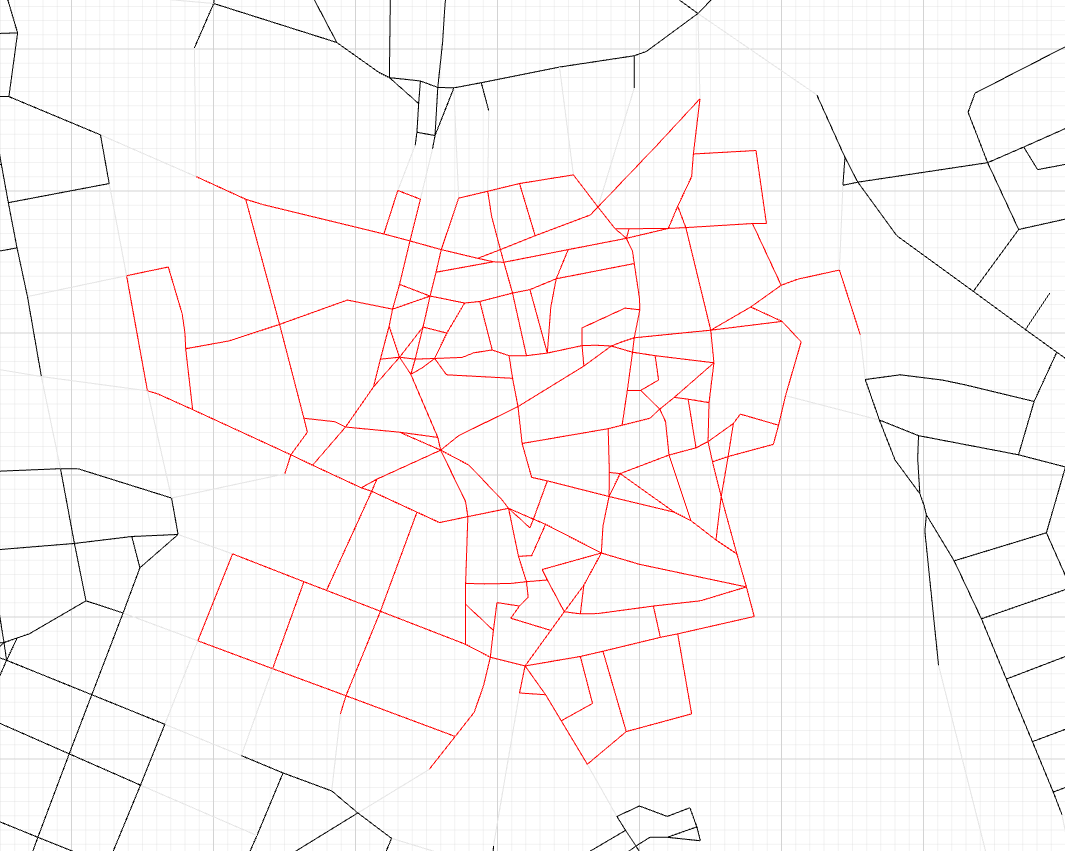
\includegraphics[width=\linewidth]{historic_district.png}
        \end{mdframed}
        \caption{Historic District of Weimar}
        \label{fig:historic_district}
    \end{subfigure}
    \par\medskip
    \begin{subfigure}[b]{0.6\textwidth}
        \begin{mdframed}[style=mdthight]
            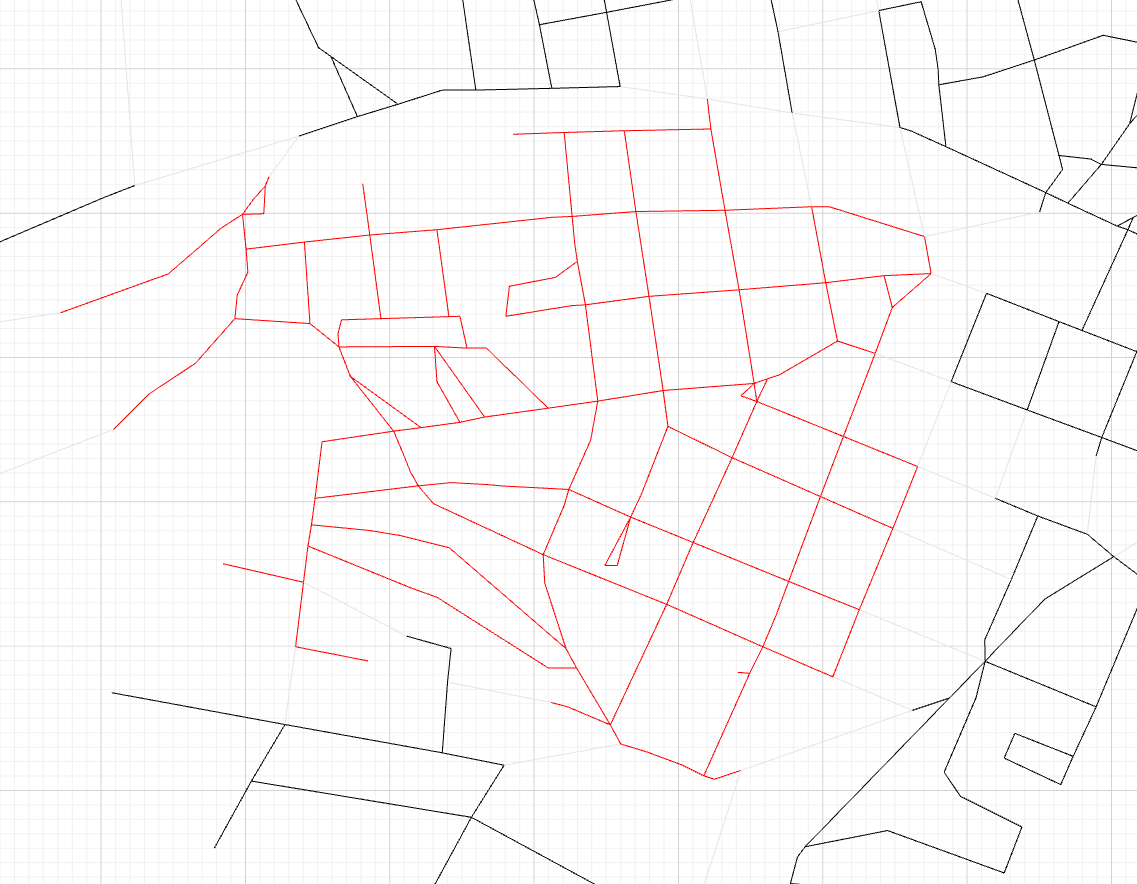
\includegraphics[width=\linewidth]{business_district.png}
        \end{mdframed}
        \caption{Business District of Weimar}
        \label{fig:business_district}
    \end{subfigure}
    \begin{subfigure}[b]{0.6\textwidth}
        \begin{mdframed}[style=mdthight]
            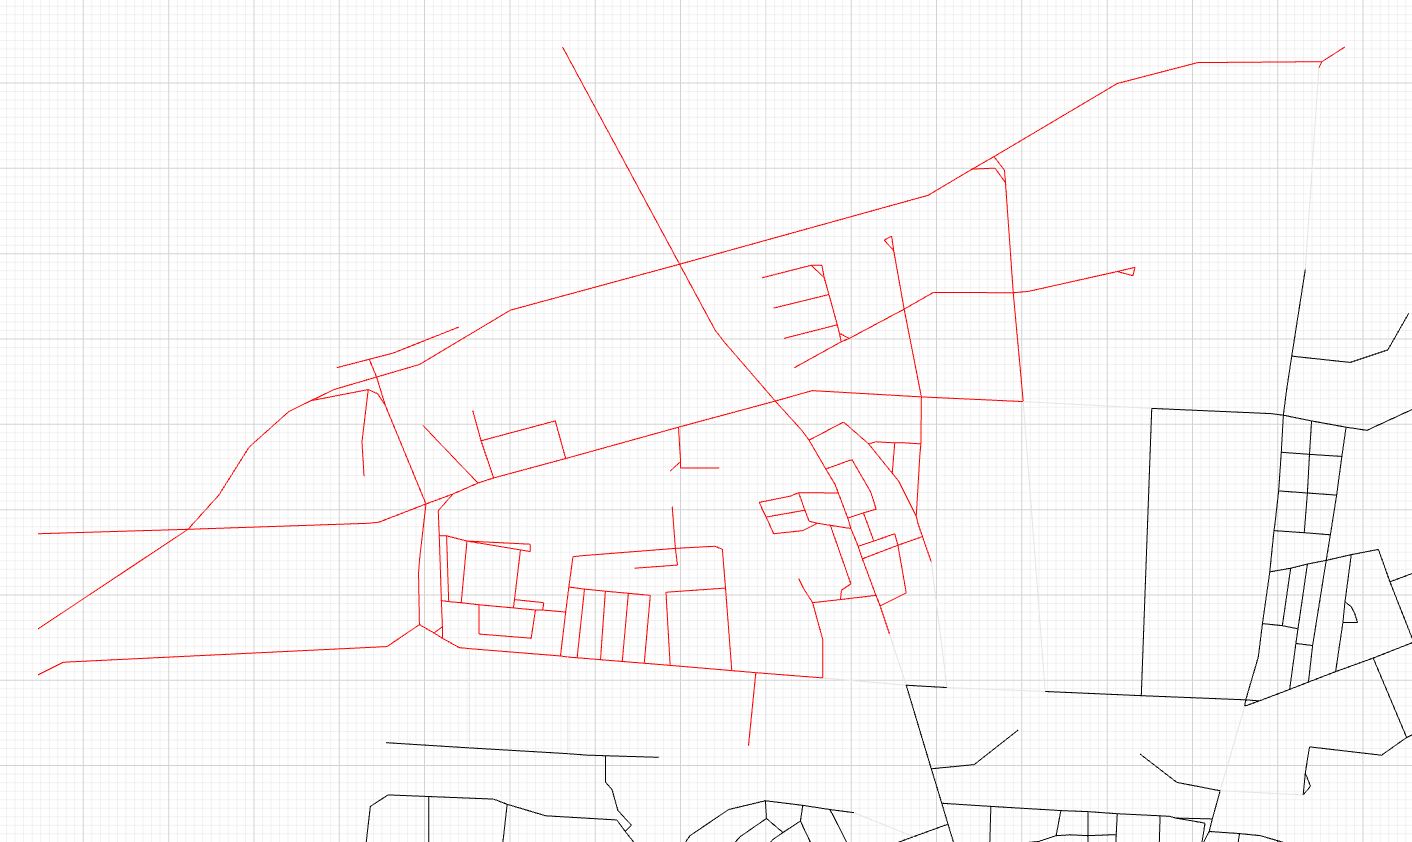
\includegraphics[width=\linewidth]{outskirts_district.png}
        \end{mdframed}
        \caption{Outskirts Area of Weimar}
        \label{fig:outskirts_district}
    \end{subfigure}
    \caption{Different areas of Weimar. Historic District (\ref{fig:historic_district}), Business District (\ref{fig:business_district}) and Outskirts Area (\ref{fig:outskirts_district})}
\end{figure}

\subsection{Business/Manhattan District}
\label{sec:businessDistinct}
If the relative block area (block area divided by surrounding circle) is high the given area is probably a business/Manhattan district. Most of the parameters are in the midrange. The image \ref{fig:business_district} with the measured data in table \ref{sec:ClusterAnalysisMeasurements} in column C2, is an example area of this district/area type.

\subsection{Outskirts Area}
\label{sec:outskits}
These areas are characterized by extreme long streets and a low connection count. As a result the density is extremely high as you can see in the example \ref{fig:outskirts_district} and the measured data in table \ref{sec:ClusterAnalysisMeasurements} in column C3. The block count is compared with a business or historic district exceptional low.

\subsection{Measured Data}
\label{sec:ClusterAnalysisMeasurements}
The following table \ref{tab:cluterAnalysisDescription} contains the parameters with additional descriptions. Extended information can be found below the table. Of every parameter the minimal (min), maximal (max), mean (average) and the median value can be calculated.

\begin{table}[h]
\begin{center}
    \begin{tabular}{ | l | l |} \hline 
        Parameter & Description \\ 
        \hline
        Total Area &  Area of the convex hull \\ \hline
        Total Length & Sum of the street length \\ \hline
        Density & Total Area divided to Total Length  \\ \hline
        
        Street Length Min/Max/Mean & Shortest/Longest/Average street length  \\ \hline
        Street Length Median & Middle value of the length dataset \\ \hline
        Street Length Variance & Sigma of the normal distribution curve of the variance \\ \hline
        
        Vertex Connections & Mean connected edges per vertex  \\ \hline
        
        Street Angle Min/Max/Mean & Smallest/Biggest/Average angle between two edges \\ \hline
        Street Angle Variance & Sigma of the normal distribution curve of the angles \\ \hline
        
        Block Count & Total number of blocks \\ \hline
        Block Area Min/Max/Mean & Shortest/Biggest/Average block area \\ \hline
        Block Area A/Ac Min/Max/Mean & Block area divided to a minimal circle around a block \\ \hline
        
        Integration Min/Max/Mean & Normalised In-Centrality \\ \hline
        Choice Min/Max/Mean & Normalised In-Betweenness-Centrality \\ \hline
    \end{tabular}
    \caption{Parameter with descriptions for table \ref{tab:measured_cluster_ratings}}
    \label{tab:cluterAnalysisDescription}
\end{center}
\end{table}

\subsubsection{Block Area}
In the paper \textit{A typology of street patterns}\citep{blockArea:2014} the method is described how cities/areas can be classified and compared by analysing the block areas instead of the streets. First the block area is calculated and then the result is divided by the circumscribed circle area.

\subsubsection{Centrality}
The parameter \textit{Integration} describes the closeness centrality. This means the normed sum of the distances from all other vertex based on te shortest path algorithm is calculated. The vertex with the lowest value must be the most central.

With \textit{Choice} the betweenness centrality is described. The approach is to calculate the shortest path between every vertex. Every time a given vertex is visited the betweenness-centrality value of the vertex is raised by one. As a result the highest measured value indicates for a vertex to be in or near the centre of a graph.

\subsubsection{Variance}
The parameter variance describes the sigma of the normal curve of the distribution function.
First of all the measured data is round to fit into a distribution function \ref{eq:distribution_function}. Then the expected value \ref{eq:expected_value} and the variance \ref{eq:variance} is calculated. Finally the standard deviation (square root of V(x)) is computed \ref{eq:standard_deviation}.
\begin{align}
\label{eq:distribution_function} 
F(x) &= P(X \leq x) =  \sum_{t\in{X}, t\leq{x}}{f(t)} \\
\label{eq:expected_value} 
E(x) &= \int\limits_{-\infty}^\infty x * f(x)dx \\
\label{eq:variance} 
V(x) &= \int\limits_{-\infty}^\infty (x - E(X))^2 * f(x)dx \\
\label{eq:standard_deviation} 
\sigma(x) &= \sqrt{V(x)}
\end{align}

\begin{table}[h]
\begin{center}
\begin{tabular}{ |l|l|l|l|l| }
    \hline
    Parmater &  
    & C1 \ref{sec:historyDistinct} 
    & C2 \ref{sec:businessDistinct} 
    & C3 \ref{sec:outskits}  \\ 
    \hline
    \multirow{4}{*}{Total} 
    & Area & 1838.05 & 1956.59 & 7802.74 \\
    & Length & 806.92 & 643.50 & 1069.81 \\
    & Density & 2.28 & 3.04 & 7.29 \\
    \hline
    \multirow{5}{*}{Street Length}
    & Min & 0.66 & 0.69 & 0.73 \\
    & Max & 9.13 & 10.68 & 38.00 \\
    & Mean & 2.72 & 3.85 & 4.82 \\
    & Median & 2.30 & 3.65 & 3.28 \\
    & Variance & 1.70 & 2.19 & 5.00 \\
    \hline
    \multirow{1}{*}{Vertex} 
    & Connections & 3.04 & 2.84 & 2.45 \\
    \hline
    \multirow{5}{*}{Street Angle} 
    & Min & 0.00 & 0.00 & 0.00 \\
    & Max & 151.80 & 358.84 & 359.80 \\
    & Mean & 119.03 & 123.75 & 137.18 \\
    & Variance & 124.68 & 131.65 & 129.47 \\
    \hline
    \multirow{5}{*}{Block} 
    & Count & 55 & 35 & 26 \\
    & Area Min & 0.01 & 0.09 & 0.00 \\
    & Area Max & 31.75 & 42.29 & 567.26 \\
    & Area Mean & 6.54 & 13.65 & 76.30 \\
    & A/Ac Min & 0.01 & 0.01 & 0.00 \\
    & A/Ac Max & 0.54 & 0.55 & 0.66 \\
    & A/Ac Mean & 0.18 & 0.23 & 0.18 \\
    \hline
    \multirow{5}{*}{Integration} 
    & Min & 0.46 & 0.48 & 0.60 \\
    & Max & 0.57 & 0.75 & 1.0 \\
    & Mean & 0.49 & 0.59 & 0.78 \\
    \hline
    \multirow{5}{*}{Choice}
    & Min & 0.00 & 0.00 & 0.00 \\
    & Max & 1.00 & 0.67 & 0.34 \\
    & Mean & 0.10 & 0.05 & 0.04 \\
    \hline
\end{tabular}
\caption{Measured results from Historic District (C1) \ref{sec:historyDistinct}, Business District (C2) \ref{sec:businessDistinct}, Outskirts Area (C3) \ref{sec:outskits} and (C4)}
\label{tab:measured_cluster_ratings}
\end{center}
\end{table}
